
% Document type and layout
\documentclass[parskip=half, titlepage=yes, 12pt, BCOR=12mm, DIV=calc]{scrartcl}

% Praeambel = definition of layout and packages
%!TeX root=Main.tex


%%%%%%%%%%%%%%%%%%%%%%%%%%%%%%%%%%%%%%%%%%%%%%%%%%%
%%%           Allgemeine Einstellungen          %%%
%%%%%%%%%%%%%%%%%%%%%%%%%%%%%%%%%%%%%%%%%%%%%%%%%%%


% Pakete für die Darstellung und Eingabemöglichkeit von Umlauten
\usepackage[T1]{fontenc}
\usepackage[utf8]{inputenc}


% Schriftarten anpassen auf helvet für seriefenlose Schrift 
% und passende Mathematik-Schrift
\usepackage{mathptmx}
\usepackage{courier}
\usepackage{microtype}     % Paket für Randausgleich

% Paket zum verwendeten erweiterter Floatoptionen
\usepackage{float}

% Pakete zum Einbinden von Bildern und Farben
\usepackage{xcolor}
\usepackage{graphicx}           


% Verwendung englischer Begriffe für automatisch generierte Worte
% wie z.B. "Contents" anstelle von "Inhaltsverzeichnis"
\usepackage[english]{babel}

% Paket um Dummy-Text/Blindtext zu erzeugen
\usepackage{blindtext}


% Mathematik Befehle und Formelsätze
\usepackage{amsmath} 
\usepackage{amssymb}
\usepackage{amsthm}
\usepackage[free-standing-units,locale = DE]{siunitx} % SI-Einheiten
\usepackage[english]{algorithm2e}     % Algorithmen
%\usepackage{MnSymbol}                % große Klammern -> falsch benutzt


% Tabellen
\usepackage{booktabs}     % Schöne Tabellen
\usepackage{supertabular} % Tabellen über mehr als eine Seite

%%%%% Literaturverzeichnis


% Literaturverzeichnis mitt BibLaTeX und Biber erstellen
\usepackage[style=numeric, sorting=none, backend=biber]{biblatex}
\addbibresource{Literature.bib}



%%%%%%%%%%%%%%%%%%%%%%%%%%%%%%%%%%%%%%%%%%%%%%%%%%%
%%%            Dokumentenlayout                 %%%
%%%%%%%%%%%%%%%%%%%%%%%%%%%%%%%%%%%%%%%%%%%%%%%%%%%


% Eigene Style-Klasse fuer eigenes Titelblatt
\usepackage{Titel}


% Allgemeine Papiergometrie
\usepackage{geometry}
\geometry{a4paper}


% Abstand der weißen Ränder
\geometry{margin=3.0cm, inner=2.5cm, outer=2.5cm} 


% Zeilenabstand auf 1,5 setzen
\usepackage[onehalfspacing]{setspace}
    \AfterTOCHead{\singlespacing}
% KOMA Klasse für europ. Layout - Wird hier nicht verwendet
  %  \KOMAoptions{DIV=last}     


% Zeit und Datumsbefehle  
\usepackage{scrdate, scrtime}   


% Erweitere Layout-Optionen
\usepackage{scrlayer-scrpage}   


% Zusätzliches Seitenlayout selbst definieren
\pagestyle{scrheadings}         


%%%%% Kopf- und Fußzeile

% Belegung von KOMA Variablen für Kopf- und Fußzeilen Gestaltung
\newcommand{\footlinetext}{\footnotesize \textsf{\color{gray}  Martin Michel, B-AMP 6  \normalsize}}

\KOMAoptions{headsepline = no, footsepline = yes}
\ihead{\headmark}
\chead{}
\ohead{}
\ifoot{\footlinetext}
\cfoot{\color{gray}\pagemark}
\ofoot{\footnotesize \textsf{\color{gray}  Radio frequency ablation with finite elements \normalsize}}



%%%%%%%%%%%%%%%%%%%%%%%%%%%%%%%%%%%%%%%%%%%%%%%%%%%
%%%   Einstellungen für Programmierquellcode    %%%
%%%%%%%%%%%%%%%%%%%%%%%%%%%%%%%%%%%%%%%%%%%%%%%%%%%


% Paket und Spezifikation der Parameter zur Darstellung 
% von Programmcode mit Courier-Schriftart
\usepackage{listings}  % Darstellung von Quellcode
\usepackage{courier}   % Schriftart laden


% Anzeigeeinstellungen für C++ Code
% Siehe Dokumentation für weitere Sprachen
\lstset{
    language=C++,
    basicstyle=\footnotesize\ttfamily,  % Standardschrift
    numbers=left,                       % Ort der Zeilennummern
    numberstyle=\tiny,                  % Stil der Zeilennummern
    %stepnumber=2,  % Abstand zwischen den Zeilennummern
    numbersep=5pt,  % Abstand der Nummern zum Text
    tabsize=2,      % Groesse von Tabs
    extendedchars=true, %
    breaklines=true,    % Zeilen werden Umgebrochen
    keywordstyle=\color{blue}\bfseries,
    frame=b,
    % keywordstyle=[1]\textbf, % Stil der Keywords
    % keywordstyle=[2]\textbf, %
    % keywordstyle=[3]\textbf, %
    % keywordstyle=[4]\textbf, \sqrt{\sqrt{}} %
    stringstyle=\color{magenta}\ttfamily, % Farbe der Strings
    showspaces=false,   % Keine Leerzeichen anzeigen 
    showtabs=false,     % Keine Tabs anzeigen 
    % xleftmargin=17pt,  % Abstände
    % framexleftmargin=17pt,
    % framexrightmargin=5pt,
    % framexbottommargin=4pt,
    commentstyle=\color{green!100!blue}\bfseries,
    %backgroundcolor=\color{grey},
    showstringspaces=true,      % Leerzeichen in Strings anzeigen
    morekeywords={__global__},  % additional language specific keywords
    morecomment=[l]
    }

    
% Syntax-Highligthing aktivieren
\lstloadlanguages{ 
    %[Visual]Basic
    %Pascal
    C,
    C++,
    %XML
    %HTML
    Matlab
    %Java
}



%%%%%%%%%%%%%%%%%%%%%%%%%%%%%%%%%%%%%%%%%%%%%%%%%%%
%%%           Layout im PDF Viewer              %%%
%%%    Muss als letztes Paket geladen werden    %%%
%%%%%%%%%%%%%%%%%%%%%%%%%%%%%%%%%%%%%%%%%%%%%%%%%%%


\usepackage{hyperref}           
\hypersetup{
    plainpages=false,
    linktocpage=true,
    breaklinks=true,
    colorlinks=true,
    linkcolor=black,%blue,
    anchorcolor=black,
    citecolor=black,%green,
    filecolor=black,%blue,
    urlcolor=black,%blue%
    pdfstartview={FitV},
    pdfview={FitH},
    pdfpagelayout={SinglePage},
    pdfpagemode={None},
}




%%%%%%%%%%%%%%%%%%%%%%%%%%%%%%%%%%%%%%%%%%%%%%%%%%%
%%%          Variablen zum Belegen              %%%
%%%%%%%%%%%%%%%%%%%%%%%%%%%%%%%%%%%%%%%%%%%%%%%%%%%


%%%%%% Variablen für Titelblatt

\DAAutor{Martin Michel}
\DATyp{Report of the application project}
\DAAutorAdresse{Keßlerplatz 12\par DE-90489 Nuremberg}
\DAFachbereich{AMP}
\DATitel{Simulation of a medical therapy \\ method with finite elements}
\DABetreuerA{Prof.\ Dr.\ rer.\ nat.\ Tim\ Kröger}
\DABetreuerB{Prof.\ Dr.\ rer.\ nat.\ habil.\ Jörg\ Steinbach}
\DABetreuerC{Prof.\ Dr.\ rer.\ nat.\ Thomas\ Lauterbach}
\DAOrt{Nuremberg}
\DAAbgabedatum{31.\,August\,2020}


\usepackage{amsthm}
\usepackage{lipsum}

%% Actual document
\begin{document}


% Title and registers
\maketitle
\tableofcontents

\clearpage

% \listoffigures
% \listoftables
% \lstlistoflistings
% \clearpage


% part 1, Introduction 

\section{Introduction to Radio Frequency Ablation}
Radio frequency ablation is a modern minimally invasive practice in surgery . In medicine it is mainly used to destroy human tissue. The two main areas of application are the medical treatment of tumours, as it destroys the malignant tissue, and also the treatment of chronic pain patients, as it can destroy nerve fibres that conduct pain signals to the brain. In the process, needles with electrodes are inserted into the patient. An external generator applies electricity and the heat generated by the electrodes increases the temperature of the tissue. The process is usually used in the temperature range of 70 to 100 degrees Celsius. A therapy session lasts for the patient from 20 minutes to several hours, depending on the need and case.
Radio Frequency Ablation (RFA) has been proven to be one of the best therapies for small tumors, which means areas smaller than 5 cm, in the human liver and kidney. The use of this treatment in modern medicine is increasing, as is the interest in research in this field. 
One of the largest branches of research is the simulation of such a therapy. Experimental research is usually based either on real patients or alternatively on animal organs such as the livers of pigs. Since experimental practice is generally very cumbersome, the interest in simulating such processes was there from the very beginning.  
With a stable and converging simulation model it is easier to try out different modifications and configurations of the process. Of course, these simulations are by no means a substitute for experimental practice, but they are a valuable addition to research. 
On a larger scale, the simulation of this process is used with virtual reality simulation programs to train physicians and surgeons in this process.\\

\begin{figure}[H]
    \centering
    \includegraphics[width=0.75\textwidth]{pictures/ra_kidney_2.jpg}
    \caption{Schematic illustration of Radio Frequency Ablation}
    \label{fig:ra_kidney_2}
\end{figure}

This is the documentation of an academic approach to numerical finite element simulation. A model for the simulation of radio frequency ablation is used as the underlying time-dependent problem.
The main purpose of this project is to study the finite element method and its convergence behaviour in an academic setting, rather than to verify a realistic simulation of radio frequency ablation. 
The underlying RFA model is described as a three-dimensional coupled system of time-dependent partial differential equations. In this investigation the model is computed in 2D space with discrete time solutions. By modeling a single needle, the original 3D domain has a rotational symmetry around the needle. The rotationally symmetric 3D model can thus be described with 2D ring elements on a cross-section and special finite element techniques. 
All algorithms were implemented with the mathematical programming tool MatLab from MathWorks.


% part 2, Main

\section{Simulation of radio frequency ablation}

\subsection{Discrete Numerical Simulation}
Physical relations can usually be described by physical laws, which in turn can be described by mathematical relations. 
Usually, the descriptions represent highly complex systems, which in turn are described by ODEs, PDEs and statistics.
In real-world physics, these models are limited by boundary conditions that allow the calculation of certain solutions of the mathematical modeling. 
In most areas of physics, with the exception of quantum mechanics and modern theoretical physics, rough models can be formulated for which concrete solutions can be found. 
Since the physics of our world is determined to a certain degree, investigations can also be carried out with the help of computer-aided simulations instead of experiments and measurements. 
Properly performed simulations can be easily modified and adapted to different models and limits. \\

In practice, the geometric dimensions of most problem descriptions are very irregular.
In many cases, there is no reasonable analytical approach to solve these problems, especially in engineering applications. For this purpose, more and more improved numerical methods have been developed in the last decades. 
Instead of a smooth analytical solution, an approximation is calculated with sufficiently high accuracy.\\

For the numerical solution of partial differential equations, the methods of finite differences, finite elements, finite volumes and boundary elements have become widely accepted in practice.
In this simulation approach, a model of radio frequency ablations is discretised and computed with common finite element techniques. \\




\subsection{About Errors in simulations and numerical approaches}

The numerical simulation of physical processes leads along the whole process from the description of the real problem up to the discrete solution to various sources of error.

\begin{itemize}
    \item Idealization errors, the discrepancy between reality and idealized reality and idealized constitutive laws and boundary conditions. In reality, physical relationships are often much more complex than the mathematical assumptions and side effects are often neglected.
    
    \item Modelling errors, the discrepancy between mathematical formulation and physical model. Often physical assumptions in the mathematical description are represented by dimensionally reduced approaches, such as linear dependencies or invariant parameters.
    
    \item  Discretization error, the discrepancy between the continuous description of the problem and the transfer to a discretized description. Discretization is in most cases merely a sufficiently accurate approximation to the continuum.
    
    \item Solution errors, caused by the use of iterative approximation methods and generally rounding errors within the scope of calculation accuracy. Beside the limited computing resources in general, it has to be considered that exact calculations are mostly not useful, because the underlying modeling also represents only an idealized estimation in the context of the error sources described above.
    
\end{itemize}


Sources of error basically cause a butterfly effect, the earlier approximations are made, the greater the inaccuracy of the simulation results. In addition, the sources of error are often in antinomic relationships to each other, i.e. the optimization of one source of error is itself in conflict with another. For example, the modeling of nonlinear dependencies requires more complex solution algorithms which in turn generate new numerical sources of error. Further information on this topic can be found in this dissertation by Sorger \cite{sorger}.


\subsection{The physics behind radio frequency ablation}
The underlying physical processes of radio frequency ablation can be described relatively straightforwardly.
Needles with electrodes (either monopolar or bipolar) are inserted into the damaged tissue. The attached electrodes create a quasi-static potential in the target tissue. Outside the target tissue, the potential is removed in a controlled manner with the help of an additionally applied mass. \\

Electrical power is generated by an external generator using the quasi-static potential. This power supply is the basis for the electrically generated energy in the area of the probes.
In principle, energy is not lost and the tissue resistance converts the energy into heat. \\

The heat generated is distributed throughout the tissue, which is why the temperature in the target area rises continuously. 
In addition, the blood circulation causes a cooling effect through heat dissipation. The controlled temperature increase in the tissue kills the damaged target tissue. The entire process is controlled from the outside to keep the temperature in the ideal target area. \\

Therefore the interesting result we are looking for is the discrete temperature distribution $\si{T}$ over time. \\

The following description is derived from a RFA model by Kröger \cite{kroeger}. This description serves to illustrate the physical relationships. An adaptation to the calculation domain $\Omega$ will follow later.

For simplicity, all material parameters are considered constant. In reality, the material parameters are strongly non-linearly dependent on both the temperature and the personal body conditions of the individual patient. Research on this aspect can be found at Stein \cite{stein} and Watanabe \cite{watanabe}. \\


The electrical energy $E_{el}(x,y,z,t)$ is calculated from the electrical power $p$.This in turn is determined by the potential $varphi$ in the calculation area. Ignoring boundaries, $\varphi$ is defined as following:
\begin{equation}
    - \nabla \cdot (\sigma(x,y,z,t) \nabla \varphi(x,y,z,t)) = 0
\end{equation}

Where $\sigma$ is the electric conductivity of the surrounding tissue. \\
The power applied by the probe is therefore obtained by the following relationship:
\begin{equation}
    p(x,y,z,t) = \sigma(x,y,z,t) \cdot |\nabla \varphi(x,y,z,t)|^2
\end{equation}

The actual potential induced by the generator can be acquired by a scaling, taking into account the non-linear behaviour of the power supply due to tissue resistance. Therefore the effective power $p_{eff} $can be modeled as following:   
\begin{equation}
    p_{eff}(t) = \frac{4 \cdot p_{setup} \cdot R_{tis}(t) \cdot R_I}{(R_{tis}(t) + R_I)^2}
\end{equation}

Where $R_{tis}$ is the tissue resistance, $R_I$ is the inner resistance of the generator, $p_{setup}$ is the initial setup power of the generator $U$ the potential difference between the electrodes.

The total power $p_{total}$ is obtained by the domain integral over the power distribution.
\begin{equation}
    p_{total}(t) = \int_{\Omega} p(x,y,z,t) dx
\end{equation}

Tissue resistance is therefore modeled as linear depending on the total power.
\begin{equation}
    R_{tis}(t) = \frac{U^2}{p_{total}(t)}
\end{equation}

From these quantities, the electric energy can be calculated.
\begin{equation}
   E_{el}(x,y,z,t) = p(x,y,z,t) \cdot \frac{p_{eff}(t)}{p_{total}(t)} = Q_{rf}(x,y,z,t)
   \label{eq:q_rfa}
\end{equation}


Since no energy is lost, the generated electrical energy becomes heat energy $Q_{rf}$ by tissue resistance. \\

The energy generated causes the temperature to rise. The exact temperature distribution $T$ is described by the well known heat equation:

\begin{equation}
    \partial_t (\rho(x,y,z,t) \cdot c(x,y,z,t,) \cdot T(x,y,z,t)) - \nabla \cdot (\lambda(x,y,z,t) \cdot \nabla T(x,y,z,t)) = Q_{total}(x,y,z,t)
\end{equation}

Referring to the parameters above, $\rho$ is the density, $c$ is the specific heat capacity and $\lambda$ represents the thermal conductivity of the tissue, which are all highly dependent on the temperature $T$. \\
The total heat energy $Q_{total}$ on the right hand side is basically the sum of all contributing heat sources and sinks. A very simplified approach leads to the following relationships:
\begin{equation}
    Q_{total} = Q_{rf} + Q_{perf}
\end{equation}

Where $Q_{rf}$ is descripted above and $Q_{perf}$ models the additional cooling effect due to blood perfusion, which is given by the following equation:
\begin{equation}
    Q_{perf}(x,y,z,t) = \nu_{perf} \cdot \rho_{blood} c_{vlood} \cdot (T_{body} - T(x,y,z,t))
    \label{q_perf}
\end{equation}
 
 Where $\nu_{perf}$ serves as an additional perfusion coefficient.

This model serves as a basis for time-dependent discrete numerical simulation. As mentioned in the beginning, the geometric calculation area is discretised on a 2D half-section, which represents an axis-symmetric 3D geometry. 


\section{Finite elements for discrete simulation}

\subsection{Elliptical problems}
The Finite Element Method essentially consists of breaking down a problem into a finite number of sub-problems and solving them as a complete system of interrelated equations. For this purpose a given geometry is covered with a mesh of polygons and decomposed into sub-areas, the finite elements. Each element is described by a variation problem and approximated by local shape functions. For elliptical problems, the system of equations is built up successively as a system of systems of equations for each individual element. The assembly is initially done without consideration of boundary conditions. These are considered by subsequent manipulation of the system of equations. Especially for this simulation the Ritz-Galerkin method is used on a two-dimensional grid with triangular elements. 

\subsection{Parabolic problems}
Parabolic problems can be solved in a similar way. This is done with a combined finite element method and a solution method for systems of ODE equations. For this purpose the parabolic problem is first considered as a simple elliptic problem without the term with the time derivative. This can then be transformed into a system of equations for the variation problem using the finite element method for elliptical problems. Subsequently, the resulting problem is used as a system of ordinary differential equations for the original problem and is solved by means of appropriate computational methods such as a Runge-Kutta method.
\begin{equation}
     M_h \cdot \underline{\dot{u}_h}(t) + K_h(t) \cdot \underline{u_h}(t) = \underline{f_h}(t) \quad \forall \; t \in [0,T]
\end{equation}
\begin{equation}
    \underline{\dot{u_h}}(t) = -M_h^{-1} K_h(t) \cdot \underline{u_h}(t) + M_h^{-1} \cdot \underline{f_h}(t) \quad \forall \; t \in [0,T]
\end{equation}
    


The resulting system of ordinary differential equations can be solved either continuously or again discretely using concrete time steps. In this simulation a time discretization is used and the implicit Euler method for ODE systems is used for the solution. A detailed description can be found in the books by Munz \cite{munz} and Loustau \cite{loustau}.


\subsection{Axial symmetrie}
In general, symmetry should be exploited in numerical methods wherever possible, thereby drastically reducing complexity and computing time. If the chosen domain is cylindrical symmetric, the calculation can be reduced from a 3D problem to an equivalent 2D cross-sectional problem. The dimension reduction results in an immense saving of computing resources.

\begin{figure}[H]
    \centering
    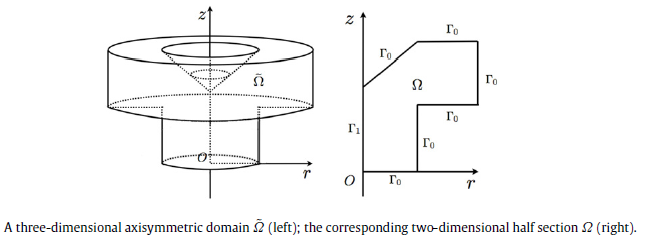
\includegraphics[width=1.0\textwidth]{projection_2D_general.PNG}
    \caption{Schematic projection on 2D half section}
    \label{projection_2D_general}
\end{figure}

A detailed description of the dimensional reduction for a finite element method for elliptic problems in a cylinder-symmetric domain can be found in the publication by Hengguang \cite{hengguang}.



\section{Discretization of PDEs}

\subsection{Computational domain}

When simulating one single probe and using homogeneous and constant material parameters, the entire calculation area is axisymmetric around the needle. To make this symmetry usable for simplifying complexity, the problem has to be adapted according to the symmetry. The partial differential equations are reduced to a 2D problem by using ring elements and cylindrical coordinates, whereby the dependence on the angle is completely eliminated. \\

The calculation area used is shown below. It is sufficient to use only half of the presented calculation area. The full cross section serves at this point for a better understanding of the geometry and is later used for plausibility checks of the simulation results.

\begin{figure}[H]
    \centering
    \includegraphics[width=0.9\textwidth]{pictures/Grid_Explanation_full.PNG}
    \caption{2D cross-section of the axis symmetric calculation domain}
    \label{fig:Grid_Explanation_full}
\end{figure}

\subsection{FEM in cylindrical Coordinates}

The equations described above refer to a Cartesian coordinate system. In order to exploit the rotational symmetry, all calculations of the domain must be adapted to cylindrical coordinates and the equations must be transformed accordingly. As an example, the Laplace operator in cylindrical coordinates is given here, which is used to describe the two partial differential equations.
 
Laplace in cartesian coordinates:
\begin{equation}
    \nabla^2 := \Delta := \frac{\partial^2}{\partial x^2} + \frac{\partial^2}{\partial y^2} + \frac{\partial^2}{\partial z^2}
\end{equation}

Laplace in cylindrical coordinates:
\begin{equation}
    \Delta := \frac{\partial^2}{\partial r^2} + \frac{1}{r} \frac{\partial}{\partial r} + \frac{1}{r^2} \frac{\partial^2}{\partial \phi^2} + \frac{\partial^2}{\partial z^2}
\end{equation}



\subsection{PDE for Electric potential}

\subsubsection{Discretization of the domain}

From a mathematical point of view, 4 different areas of the computational domain are of interest:
\begin{itemize}
    \item Inner area between the boundaries
    \item Electrodes 
    \item Rest of the sample and the outer boundaries
    \item Artificial boundary on the rotation axis
\end{itemize}

As mentioned above, only constant material parameters are assumed. This results in essential simplifications for the further calculation.

\subsubsection{Inner Domain}

The electrical potential in the inner domain behaves as described above:
\begin{equation}
    - \nabla \cdot (\sigma(x,y,z,t) \nabla \varphi(x,y,z,t)) = 0
\end{equation}

As sigma is assumed to be constant the following relation is valid:
\begin{equation}
    \nabla \cdot \sigma = 0
\end{equation}

Trivially this equation is now independent of $\sigma$, so $\sigma$ can be easily removed. The partial differential equation becomes the Laplace equation and $\varphi$ becomes time independent.
\begin{equation}
    - \Delta \varphi(x,y,z) = 0
\end{equation}

Adapted to the domain, the axis symmetry is exploited by using cylindrical coordinates.
\begin{equation}
    - \Delta \varphi(r,\phi,z) = - \frac{1}{r} \frac{\partial \varphi}{\partial r} - \frac{\partial^2 \varphi}{\partial r^2} - \frac{1}{r^2} \frac{\partial^2 \varphi}{\partial \phi^2} -      \frac{\partial^2 \varphi}{\partial z^2}  = 0
\end{equation}

Because of the axial symmetry, the solution for $\varphi$ is independent of the angle $\phi$. The PDE is thus reduced by one dimension. 
\begin{equation}
    - \nabla  ( \sigma \cdot \nabla \varphi(r,\phi,z)) \overset{!}{=} - \Delta \varphi(r,z) = - \frac{1}{r} \frac{\partial \varphi}{\partial r} - \frac{\partial^2 \varphi}{\partial r^2} - \frac{\partial^2 \varphi}{\partial z^2} = 0
\end{equation}

To keep the following descriptions clearer, the explicit specification of coordinates is omitted. $\varphi$ is dependent on $r$ and $z$ unless otherwise specified.

\subsubsection{Electrodes}

The potential difference at the electrodes is fixed by definition. For the calculations the potential is defined as $\pm 1$ arbitrarily chosen. Since only one needle is modeled, it has a positive and negative electrode each.
\begin{equation}
    \varphi = \pm 1
\end{equation}

Other values are also possible in principle, but are not useful for this modelling.

\subsubsection{Outer boundary}

To make the calculation as reasonable as possible, it is assumed that all other outer edges have natural Neumann boundary conditions for the electric potential $\varphi$. Although this does not exactly reflect the physical conditions of the potential, it is very appropriate in the context of the simplifications made.
\begin{equation}
    n \cdot \nabla \varphi = 0
\end{equation}

In addition to the electrodes, a mass is applied in the RFA treatment to nullify the potential in the outer regions. This behavior is simulated by assuming fixed Dirichlet values at the lower edge.
\begin{equation}
    \varphi = 0
\end{equation}

Neither the Neumann nor the Dirichlet conditions correctly reflect the underlying physics, but are rather rough simplifications.
Since further simplifications in the modeling were already made in the run-up, especially by the unrealistic assumption of constant material parameters, these simplifications of the boundary conditions are within the range of acceptable errors.


\subsubsection{Rotation axis}

The edge on the symmetry axis is purely artificial and a product of dimensional reduction. For reasons of maintaining symmetry, it is easy to see that natural boundary conditions apply here.
A formal and detailed investigation of this statement can be found in the publication of Hengguang \cite{hengguang}. 

- \begin{equation}
    n \cdot \nabla \varphi = 0
\end{equation}



\subsection{Calculation of electrical energy}

With the introduced descriptions $\varphi$ is calculated for each discrete point. If $\varphi$ is known, the electrical power $p$ can be calculated according to the above mentioned physical relations (\ref{eq:q_rfa}). Since $\varphi$ and all other parameters are time independent, the electrical power is also time independent. This allows to calculate the generated electrical energy $Q_{rf}$ as a linear dependence on time for each point in time. As time progresses, the total electrical energy introduced into the system accumulates. 

\subsection{PDE for temperature Distribution}

\subsubsection{Discretization of the problem}

From physics above, the temperature distribution is modeled by the heat equation: 
\begin{equation}
    \partial_t (\rho c T) - \nabla \cdot (\lambda \nabla T) = Q
\end{equation}

The heat equation is a well known parabolic partial differential equation. \\

Since the material parameters $\rho$, $c$ and $\lambda$ are assumed to be constant, the temperature $T(r,z,t)$ and thermal energy $Q(r,z,t)$ remain as variables of interest.

In the temperature range of radiofrequency ablation, $c$ and $\lambda$ are particularly nonlinearly dependent on the respective temperature, this is especially due to the phase change of water from liquid to gaseous. Vaporized water has a completely different heat capacity and thermal conductivity, the corresponding transition is smooth and not abrupt. However, modeling the phase change of water and the corresponding heat capacity leads to great numerical challenges in practice. It is a reasonable compromise to model at least the temperature dependence of lambda, which leads to the following description in cylindrical coordinates:
\begin{equation}
    \rho c \frac{\partial T}{\partial t} -  \frac{d\lambda}{dT} \left[ \left( \frac{\partial T}{\partial r} \right)^2 + \left( \frac{\partial T}{\partial z} \right)^2 \right] - \lambda \left( \frac{\partial^2 T}{\partial r^2} + \frac{1}{r} \frac{\partial T}{\partial r} + \frac{\partial^2 T}{\partial z^2} \right) = Q
\end{equation}

A model with variable thermal conductivity is used in the work of Watanabe \cite{watanabe}.

In order to keep this simulation on an academic scale, $\lambda$ is still considered constant. This leads to the following simplification:
\begin{equation}
    \rho c \frac{\partial T}{\partial t} - \lambda \left( \frac{\partial^2 T}{\partial r^2} + \frac{1}{r} \frac{\partial T}{\partial r} + \frac{\partial^2 T}{\partial z^2} \right) = Q
\end{equation}

As mentioned in the physical description, the right side is the sum of all thermal energies.
\begin{equation}
    Q_{total} = Q_{rf} + Q_{perf}
\end{equation}

Since the material parameters are constant, $Q_{perf}$ can be evaluated as linear dependence of T for each time step, see equation (\ref{q_perf}). 

\subsubsection{Needle}

If we assume that the probe is cooled from the outside, it is a simple and relatively accurate assumption to take the body temperature as a constant temperature for the probe.
\begin{equation}
    T = T_{body} \
\end{equation}

Normally the body temperature is about $\cong$ 37 degrees Celsius or 310.15 degrees Kelvin. For a simulation of an uncooled probe, another simple approach is to model the behavior of the needle like the behavior at the other outer boundaries.

\subsubsection{Outer boundary}

Assuming that there are no external disturbances, the natural boundary conditions are the correct assumption for the heat equation.
\begin{equation}
    n \cdot \nabla \, T = 0
\end{equation}

For simplicity, this assumption is also used to model an uncooled probe.

The following describes how the PDE models for $\varphi$ and $T$ are handled in the context of the finite element method and can be numerically evaluated at discrete points.


\section{Applied FEM technologies}

\subsection{Weak solutions}
\subsubsection{Electric potential}

For the Ritz-Galerkin method, it is mandatory to transform the PDEs above into weak formulations. Poisson's equation for reference is given as follows:
\begin{equation}
    a_w(u,v) := \int_{\Omega} (\partial_r u \partial_r v + \partial_z u \partial_z v) r drdz = \int_{\Omega} f v r dr dz
\end{equation}
\begin{align}
    u \in H_r^1(\Omega) \cap \{v|_{\Gamma_{0}} &= 0 \} 
    \label{trial_functions1}\\
    v \in H_r^1(\Omega) \cap \{v|_{\Gamma_{0}} &= 0 \}     
    \label{trial_functions2}
\end{align}

More information about the above transformation for Laplace's equation as well as a detailed proof of conformity can be found in the work of Hengguang \cite{hengguang}. \\

This formulation leads analogously to the following description of the electric potential $\varphi$ for the inner domain: 
\begin{equation}
    a_w(u,v) := \int_{\Omega} (\partial_r u \partial_r v + \partial_z u \partial_z v) r drdz = 0 
\end{equation}

Using the same trial functions as described above (\ref{trial_functions1}) (\ref{trial_functions2}).  

\subsubsection{Temperature Distribution}

The temperature distribution as a hyperbolic problem can be described as a fully discrete substitute problem by discontinuous Galerkin FEM. The variation problem consists of a local discretization of the Laplace problem and a subsequent discretization in the time dimension.   

A weak formulation of the problem can be described as follows: \\
We are looking for $u(r,z,t) \in V_{g1}$ with $\Dot{u} \in L_2(\Omega)$ for almost every $t \in (0,T)$, so  
\begin{equation}
    (\Dot{u},v)_0 + a(t;u,v) = \langle F(t),v \rangle \; for \; all \; v \in V_0    
\end{equation}
and for almost every $t \in (0, T)$ is the condition given as 
\begin{equation}
    (u(r,z,0),v)_0 = (u_0,v)_0 \; for \; all \; v \in V_0
\end{equation}

The formal description is given by 
\begin{align*}
    (\Dot{u},v)_0 &= \int_{\Omega} \Dot{u}(r,z,t)v(r,z) drdz = \int_{\Omega} \frac{\partial u(r,z,t)}{\partial t} v(r,z) drdz, \\
    a(t;u,v) &= \int_{\Omega} \left[ \lambda_1(r,z,t) \frac{\partial u}{\partial r} \frac{\partial v}{\partial r} + \lambda_2(r,z,t) \frac{\partial u}{\partial z} \frac{\partial v}{\partial z} \right] \cdot r \cdot drdz + \int_{\Gamma_3} \alpha(r,z,t)u(r,z,t)v(r,z) ds, \\
    \langle F(t),v \rangle &= \int_{\Omega} f(r,z,t)v(r,z) drdz + \int_{\Gamma_2} g_2(r,z,t)v(r,z) ds + \int_{\Gamma_3} \alpha(r,z,t)u_A(r,z,t)v(r,z) ds, \\
    V_{g_1} &= \{u \in H^1(\Omega) : u = g_1 \; in \;  \Gamma_1 \; for \; almost \; every \; t \in (0,T) \} \\
    V_0 &= \{ v \in H^1(\Omega) : v = 0 \; in \; \Gamma_1 \}
\end{align*}

Adapted for the temperature distribution, assuming $\lambda$ and all material parameters are constant, the weak formulation can be described as follows: 

\begin{equation}
    a_w(t;u,v) := \int_{\Omega} \rho c (\partial_t u \cdot v) r drdz + \int_{\Omega} \lambda (\partial_r u \partial_r v + \partial_z u \partial_z v) r drdz = \int_{\Omega} f v r dr dz
\end{equation}

Using the same trial functions as described above (\ref{trial_functions1}) (\ref{trial_functions2}).  \\

For further information on the fully discrete weak formulation, please refer to the work of Jung \cite{jung}.


\subsection{Discretization / Triangulation}

A triangular grid is used for the calculations. Triangles are generally more flexible to adapt to the geometry than rectangles. An initial coarse grid triangulation is done by hand and then the elements are further refined with an algorithm as desired. A triangle can easily be broken down into 4 smaller triangles. For the simulation, both coarse and fine grids are used and the results are examined. Finer elements are generally better suited for the calculation accuracy of the numerical PDE solution, but especially when calculating the numerical gradient, too fine elements can lead to errors. 

Because of the symmetry it is sufficient to perform the calculations on half of the cross-section. For comparison and plausibility checks, some calculations are also performed on the full cross-section. Since the calculation results on the full cross-section should theoretically be completely symmetrical, a rough visual check for numerical errors can be made in advance.


\begin{figure}[H]
    \centering
    \includegraphics[width=0.8\textwidth]{pictures/triangulation_full.PNG}
    \caption{Triangulation on the full cross-section}
    \label{fig:triangulation_full}
\end{figure}

\begin{figure}[H]
    \centering
    \includegraphics[width=0.8\textwidth]{pictures/triangulation_halved_coarse.PNG}
    \caption{Triangulation on the halved cross-section}
    \label{fig:triangulation_halved}
\end{figure}


\subsection{Assembling system of equation}

The assembly of the equation system is done element by element. To approximate the solution to the variation formulation, linear regressions functions are used. The calculation of the individual elements is performed on normalized reference triangles using the affin linear transformation.

Linear regression functions in two space dimensions on reference triangle:
\begin{align}
    \phi_1(\xi, \eta) &= 1 - \xi - \eta \\
    \phi_2(\xi, \eta) &= \xi \\
    \phi_2(\xi, \eta) &= \eta 
\end{align}


\subsection{Error estimations}

Error estimations concerning the elements for finite element methods are usually done using the H1 norm, L2 norm or the energy norm. The analytical solution of the problem is unknown in this case, which makes a safe estimation difficult. Nevertheless, the geometric error can be estimated relatively well by calculating the same partial area with different element sizes and comparing the results. If the difference is too large, the calculation should be continued on a finer grid with more elements. 

In a similar way the error in the time step size can be estimated. The same time interval is calculated once with step size in one step and once with halved step size in two steps. By comparing the error norms for both methods it can be roughly estimated whether the time step is too coarse for the stiff problem and should be reduced.


\newpage


\section{Other numerical aspects }


\subsection{Surface integral}
The surface integral over the individual elements is required for the element by element assembly of the systems of equations. The computation of these takes place on discrete Gauss quadrature points. In this simulation, either 3 or 7 base points were used for the quadrature. More base points increase the calculation effort, but generally result in more precise calculation results. A detailed reference of the method used can be found in the book by Jung \cite{jung}.

\subsection{Numerical gradient on discrete points}
In the Ritz-Galerkin algorithm, the applied trial functions approach the solution of the variation problem. The numerical gradient thus approximately corresponds to the gradients of the approach functions on the element. For this implementation only linear functions were used, accordingly the numerical gradient is constant for each element. In order to obtain an exact numerical result for the gradient on the discrete grid points, a mean value was calculated from the constant gradients of the surrounding elements.


\subsection{Troublesome neighbours}
The joint use of Dirichlet and Neumann boundary conditions can lead to problems at individual points, specifically at the corners of Dirichlet edges to a Neumann edge. In the simulation this problem occurs concretely at the electrodes. Dirichlet nodes are treated by manipulating the equation of the node to a trivial problem. Dirichlet boundary conditions have a higher priority, therefore the common corner node is treated as a Dirichlet boundary condition. Before manipulating the matrix, the result of a matrix-vector multiplication with non-manipulated data is subtracted from the affected parts of the equation system on the right side. This compensates side effects of the following modification. The right side of the equation is set to the Dirichlet value and the corresponding matrix entry gets the value 1. All other variables of the affected row and column vector are set pragmatically to the value 0. This pragmatic procedure is exact for a Dirichlet node and does not require any calculation. However, this procedure has a very negative effect on an adjacent Neumann edge. By artificially modifying the system of equations, the equation for the directly adjacent Neumann node is invalidated. The calculation of the node thus delivers an undefined result. To overcome this problem, it has proved to be useful to ignore the calculated result for this concrete node and to interpolate a substitute result by weighting the results of neighboring nodes. This special implementation has obvious flaws, but achieves relatively good results in practice.



% < Section 7 Applied simulation >


\section{Applied simulation}

\subsection{Reference data}
In order to be able to perform a meaningful simulation, it is necessary to find suitable reference numbers for all variables used. For the determination of material parameters the measurement results from the investigations of Stein \cite{stein} were used. For the description of the electrical generator setup a large number of configurations can be used for this investigation. Concrete data on devices that are commonly used in medical practice can be found in Padma's publication \cite{padma}. 

\subsection{Solving the PDEs}
The electric potential $\varphi$ and the electric power $p$ are calculated in advance, because they are time independent. Therefore, the electrical energy $Q_{rf}$ can easily be obtained by multiplying the power by the step size of the time discretization. Since the thermal equation is inherently very stiff, the implicit Euler method for matrices is used to calculate the discrete solution. For each time step the temperature equation is recomposed and calculated. This results in a coherent time dependent simulation.


\subsection{Graphical output}
The calculated 2D data for $\varphi$, the electrical power and the temperature distribution for each time step can easily be visualized on a 3D plot. Since the calculated cross-section solutions are axisymmetric, the calculated values are valid for every angle $\phi$. From this, a 3D reconstruction can be easily generated by defining concrete angle points. After retransforming the generated solution into cartesian coordinates, the 3D geometry can be visualized on a 4D plot with color gradient depending on the numerical solution.

\newpage

% < Section 8 Numerical results >

\section{Numerical results}

In the following the numerical simulation results are presented. The calculations were performed with different element sizes and time step sizes on both the half and the whole cross-section. In the MatLab source code all results can be recalculated and further modified in their configuration. Depending on element size and time step size the expected calculation time is between some seconds and several minutes. \\

In principle, all calculation results are qualitatively within the expected range. The calculated solutions are reasonably smooth and on sufficiently fine grids with low error tolerance. For a comparison of the plausibility of the results please refer to th.e published results of a very similar simulation with accompanying experiments by Watanabe \cite{watanabe}.

As expected, the electrical potential is maximum at the electrodes and drops very quickly in the surrounding computing area. In the following picture the calculation was performed without additional mass as boundary condition, therefore the potential at the edge is not nullified. Since only the gradient of $\varphi$ is decisive for the electrical power, the peak power lies between the electrodes.

\\

\begin{figure}[H]
    \centering
        \includegraphics[width=0.8\textwidth]{pictures/phi_2D_sideview.PNG}
        \caption{Time-independent numerical solution for $\varphi$ on a halved 2D cross-section}
        \label{phi_2D_sideview}
\end{figure}


\begin{figure}[H]
    \centering
        \includegraphics[width=0.8\textwidth]{pictures/phi_2D_topview.PNG}
        \caption{Topview of the solution for $\varphi$ on the halve grid}
        \label{phi_2D_topview}
\end{figure}



\begin{figure}[H]
    \centering
    \includegraphics[width=0.8\textwidth]{pictures/phi_3D.PNG}
    \caption{3D reconstruction of the numerical solution for $\varphi$}
    \label{phi_3D}
\end{figure}


 The electrical power is calculated using the numerical gradient of $\varphi$.  

\begin{figure}[H]
    \centering
    \includegraphics[width=0.75\textwidth]{pictures/numericalGradient_2D.PNG}
    \caption{Numerical gradient of the solution for $\varphi$}
    \label{numericalGradient_2D}
\end{figure}

The applied electrical energy is greatest around the area between the electrodes. 

\begin{figure}[H]
    \centering
    \includegraphics[width=0.75\textwidth]{pictures/effectiveEnergy_2D.PNG}
    \caption{Effective energy applied by the probe in one second}
    \label{effectiveEnergy_2D}
\end{figure}


Also the temperature calculation is generally as expected. Over time, the temperature increases slowly but steadily as continuous electrical energy is added to the system by the probe. The perfusion counteracts the temperature increase with a cooling effect. The calculations were performed over a calculated period of about 4 minutes. In the peak range, the temperature in this area rose to around 90 degrees Celsius. Temperatures above this level are usually regulated externally during RFA treatment in order not to exceed the target range. In addition, the phase change of the water must be increasingly taken into account. Both circumstances were not considered in the model, which means that a calculation over a longer period of time would no longer be appropriate.

\\

\begin{figure}[H]
    \centering
    \includegraphics[width=0.9\textwidth]{pictures/temp_2D_240sec.PNG}
    \caption{Temperature distribution after 240 seconds on a coarse halved cross-section}
    \label{temp_2D_240sec}
\end{figure}


\begin{figure}[H]
    \centering
    \includegraphics[width=0.9\textwidth]{pictures/temp_2D_240sec_finer_full.PNG}
    \caption{Temperature distribution after 240 seconds on a fine grid}
    \label{temp_2D_240sec_finer_full}
\end{figure}


\begin{figure}[H]
    \centering
    \includegraphics[width=0.9\textwidth]{pictures/temp_3D_240sec_fine.PNG}
    \caption{3D reconstruction of the temperature distribution after 240 seconds}
    \label{temp_3D_240sec_fine}
\end{figure}



% < Section 9 Summary and outlook >

\section{Summary and outlook}

\subsection{Project Summary}
\subsubsection{A humble simulation}
One could argue, that it is a waste of time to write a numerical simulation from scratch. There are already many very useful software solutions for numerical simulations and these kind of problems in general. Therefore there is usually no need to write your own detailed implementation of the underlying algorithms. \\

However, creating your own scripts and implementations helps to understand numerical problems and sources of error in this type of modeling at all. Even all commercial software is based on algorithms of this kind. Dealing with these problems on one's own greatly improves the ability to use these software products effectively and write great simulations.\\

There can be no good software developer who does not understand how a computer processes numbers. Similarly, this academic approach trains the understanding of numerical simulation. I think, everybody who deals with finite elements should have implemented such algorithms himself at some point. \\

\subsubsection{Strengths and flaws}
It is appropriate at this point to draw a conclusion about the results achieved. \\
Basically the simulation can be regarded as quite good for a study project. 
The numerical results are in good agreement with the general expectation. The calculations converge relatively reliably with reasonable choice of variables.
The chosen implementation is flexible and can therefore easily be adapted to more complex approaches and models. \\
However, the chosen model is far too simplified to be a realistic representation of the conditions of an actual RFA treatment. Further planned modifications are interesting from a mathematical point of view, but would not significantly change the results of the simulation and thus its validity.


\subsubsection{Future modifications}
I plan to expand this project in the future and let the chosen model mature. The described material parameters are in reality strongly non-linearly dependent on the temperature and the surrounding factors. An improved parameterization of these should lead to much more realistic simulation results. Especially the evaporation of water and a more complex formulation of blood perfusion should be considered. Subsequently, more complex and more realistic boundary conditions should be chosen. 
The simulation of a second needle and monopolar probes would also be conceivable. The underlying algorithm can basically be adapted to three-dimensional problems.

%\subsection{State of the current Research}
%- Research in the simulation of medical therapy methods \\
%- TODO \\


\subsection{Other FEM software}

There is a lot of great commercial FEM software available to solve problems of this kind. Matlab, the tool used for this numerical simulation, offers its own PDE toolbox with corresponding libraries with efficient implementation of almost all aspects for solving partial differential equations.

In addition, there are numerous powerful simulation tools, which also offer additional features such as built-in geometric modelers and graphical user interfaces. COMSOL Multiphysics and ANSYS are two of the most widely used tools of their kind in modern industry.

Aside from that, there are a number of powerful free open source software projects that provide a number of highly optimized library functions. Worth mentioning here are the FEniCS project and FreeFEM.


\newpage


%% Literature register using .bib file
\clearpage
\nocite{*}
\printbibliography

\newpage

%% last part, appendix
% \appendix

% %!TeX root=Main.tex

% Dieses File ist für den Anhang
% Hier kann potenzieller Quellcode generiert werden
% Sowie zusätzliche Bilder usw eingefügt werden
% Wird nicht für alle Versuche benötigt werden

\section{Source code Visual C++}

\lstset{language=C++,
                basicstyle=\ttfamily,
                keywordstyle=\color{blue}\ttfamily,
                stringstyle=\color{red}\ttfamily,
                commentstyle=\color{gray}\ttfamily,
                morecomment=[l][\color{orange}]{\#}
}

\begin{lstlisting}[caption={[Demo] For loop to print numbers from 1 to 10}]
// Print numbers from 1 to 10
#include <stdio.h>
int main() {
  int i;
  for (i = 1; i < 11; ++i)
  {
    printf("%d ", i);
  }
  return 0;
}
\end{lstlisting}


\section{Source code MatLab}

\Large{TODO}
 

\end{document} 